\documentclass[margin=5mm]{standalone}
\usepackage{tikz}

\tikzstyle{block} = [rectangle, draw, thick, minimum width=1.5cm, minimum height=1cm]
\tikzstyle{channel} = [circle, draw, thick, radius=0.25cm]

\begin{document}
    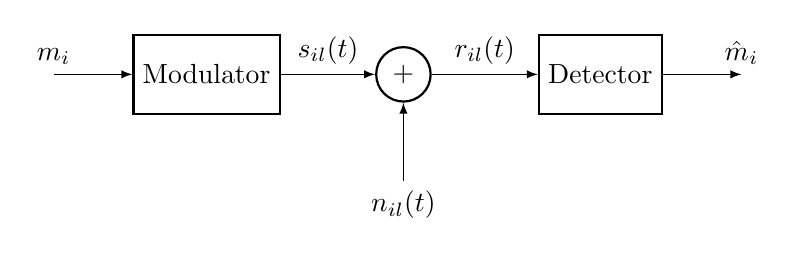
\begin{tikzpicture}[node distance=2.5cm, >=latex]
        \node[block] (modulator){Modulator};
        \node[channel, right of = modulator](channel){$+$};
        \node[block, right of = channel] (detector){Detector};

        \draw[->] (modulator) -- node[midway, anchor=south]{$s_{il}(t)$} (channel);
        \draw[->] (channel) -- node[midway, anchor=south]{$r_{il}(t)$} (detector);
        \draw[<-] (modulator.west) -- ++(-1cm, 0cm) node[anchor=south]{$m_i$};
        \draw[<-] (channel.south) -- ++(0cm, -1cm) node[anchor=north]{$n_{il}(t)$};
        \draw[->] (detector.east) -- ++(1cm, 0cm) node[anchor=south]{$\hat{m}_i$};
    \end{tikzpicture}
\end{document}
